\documentclass[12pt,a4paper]{report}

\usepackage[utf8]{inputenc} % Codificação do arquivo
\usepackage[T1]{fontenc}    % Codificação da fonte
\usepackage[brazil]{babel}
\usepackage{graphicx,url}
\usepackage[top=2cm, bottom=2cm, left=2cm, right=2cm]{geometry}
\usepackage{hyperref}
\usepackage{cmap} % Mapear caracteres especiais no PDF
\usepackage{enumitem} % Para personalizar listas
\usepackage{amsmath} % Melhor suporte matemático
\usepackage{adjustbox} % Para ajustar o tamanho de imagens
\usepackage{float} % Para posicionar imagens

\hyphenpenalty=5000 % Evitar hifenização
\tolerance=1000     % Evitar ultrapassar margens

\begin{document}
	\begin{center}
		{\Large Universidade Federal de Uberlândia - UFU}
		
		Bacharelado em Sistemas de Informação
		
		\textbf{FACOM32504 - Redes de Computadores - 2024/2}
		
		\textbf{Arthur Fernandes - 11911BCC059}
	\end{center}
	
	\vspace{10pt}

	\begin{center}
		{\LARGE \textbf{Relatório 3 \\ \vspace{10pt} Domain Name System (DNS)}}
	\end{center}
	
	\vspace{10pt}
	
	\begin{figure}[ht]
		\centering
		
\includegraphics[width=0.3\textwidth]{ufu.png}
		\caption{Logo da UFU.}
		\label{fig:logoUFU1}
	\end{figure}

	\begin{enumerate}
		\item Execute o \texttt{nslookup} para obter o endereço IP de um servidor Web do Indian Institute of Technology em Bombaim, Índia: \texttt{www.iitb.ac.in}. Qual é o endereço IP desse servidor?
		
		\textbf{Resposta:} 

		\begin{figure}[H]
			\centering
			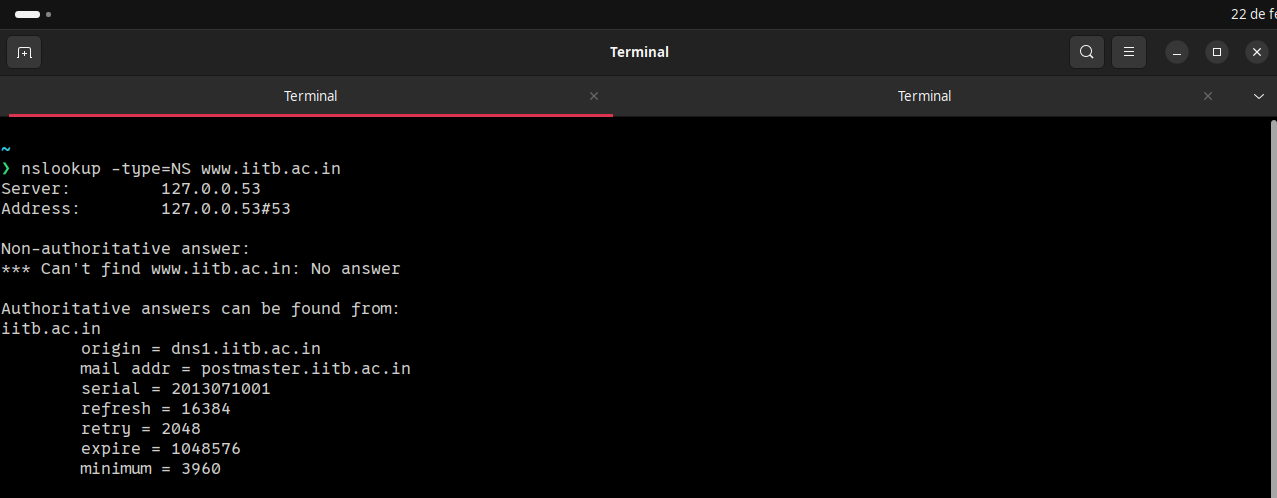
\includegraphics[width=1\textwidth]{q1.png}
			\caption{nslookup para o servidor www.iitb.ac.in (Questão 01)}
			\label{fig:versaoHTTP}
		\end{figure}

		\item Qual é o endereço IP do servidor DNS que forneceu a resposta para o comando \texttt{nslookup} da questão 1?
		
		\textbf{Resposta:} 

		\item A resposta do comando \texttt{nslookup} da questão 1 foi obtida de um servidor DNS authoritative ou non-authoritative?
		
		\textbf{Resposta:} 

		\item Execute o comando \texttt{nslookup} para determinar os servidores DNS autorizados para uma universidade na Europa.
		
		\textbf{Resposta:} 

		\item Localize a consulta DNS e as mensagens de resposta. Essas mensagens são enviadas via UDP ou TCP?
		
		\textbf{Resposta:} 

		\item Qual é a porta de destino da mensagem de consulta DNS? E qual é a porta de origem da mensagem de resposta DNS?
		
		\textbf{Resposta:} 

		\item Para qual endereço IP é enviada a mensagem de consulta DNS? Utilize o comando \texttt{ipconfig} para verificar o endereço IP do seu servidor DNS local. Esses dois endereços IP são iguais?
		
		\textbf{Resposta:} 

		\item Analise a mensagem de consulta DNS: qual é o “tipo” de consulta realizada? A mensagem de consulta contém alguma “resposta”?
		
		\textbf{Resposta:}

		\item Analise a mensagem de resposta DNS: quantas “respostas” são fornecidas e o que cada uma delas contém?
		
		\textbf{Resposta:}

		\item Considere o pacote TCP SYN subsequente enviado pelo seu host. O endereço IP de destino desse pacote corresponde a algum dos endereços IP apresentados na mensagem de resposta DNS?
		
		\textbf{Resposta:}

		\item A página base disponível em \url{http://gaia.cs.umass.edu/kurose_ross/} faz referência à imagem \url{http://gaia.cs.umass.edu/kurose_ross/header_graphic_book_8E_2.jpg}, sendo ambas hospedadas em \texttt{gaia.cs.umass.edu}.
		
		\begin{enumerate}
			\item Qual é o número do pacote no rastreamento da solicitação HTTP GET inicial para o arquivo base?
			
			\textbf{Resposta:}

			\item Qual é o número do pacote no rastreamento da consulta DNS realizada para resolver gaia.cs.umass.edu, permitindo o envio da solicitação HTTP inicial para o endereço IP correspondente?
			
			\textbf{Resposta:}

			\item Qual é o número do pacote no rastreamento da resposta DNS recebida?
			
			\textbf{Resposta:}

			\item Qual é o número do pacote no rastreamento da solicitação HTTP GET para o objeto de imagem?
			
			\textbf{Resposta:}

			\item Qual é o número do pacote referente à consulta DNS efetuada para
			
			\textbf{Resposta:}
		\end{enumerate}

		\item Qual é a porta de destino para a mensagem de consulta DNS? E qual é a porta de origem da mensagem de resposta DNS?
		
		\textbf{Resposta:}

		\item Para qual endereço IP é enviada a mensagem de consulta DNS? Esse endereço IP corresponde ao do seu servidor DNS local padrão?
		
		\textbf{Resposta:}

		\item Analise a mensagem de consulta DNS: qual é o “tipo” de consulta efetuada? A mensagem de consulta contém alguma “resposta”?
		
		\textbf{Resposta:}

		\item Analise a mensagem de resposta DNS: quantas “respostas” são fornecidas e o que cada uma delas contém?
		
		\textbf{Resposta:}

		\item Para qual endereço IP é enviada a mensagem de consulta DNS? Esse endereço IP corresponde ao do seu servidor DNS local padrão?
		
		\textbf{Resposta:}

		\item Analise novamente a mensagem de consulta DNS: qual é o “tipo” de consulta efetuada? A mensagem de consulta contém alguma “resposta”?
		
		\textbf{Resposta:}

		\item Analise a mensagem de resposta do DNS:
		
		\begin{enumerate}
			\item Quantas respostas estão presentes?
			
			\textbf{Resposta:}

			\item Quais informações estão contidas em cada uma dessas respostas?
			
			\textbf{Resposta:}

			\item Quantos registros de recursos adicionais foram retornados?
			
			\textbf{Resposta:}

			\item Quais informações adicionais estão incluídas nesses registros?
			
			\textbf{Resposta:}
		\end{enumerate}

		\item Para qual endereço IP é enviada a mensagem de consulta DNS? Esse é o endereço IP do seu servidor DNS local padrão? Caso contrário, a que endereço IP ele corresponde?
		
		\textbf{Resposta:}

		\item Analise a mensagem de consulta DNS: qual é o “tipo” de consulta efetuada? A mensagem de consulta contém alguma “resposta”?
		
		\textbf{Resposta:}

		\item Analise a mensagem de resposta DNS: quantas “respostas” são fornecidas e o que cada uma delas contém?
		
		\textbf{Resposta:}
		
	\end{enumerate} 

\end{document}
